\let\negmedspace\undefined
\let\negthickspace\undefined
\documentclass[journal]{IEEEtran}
\usepackage[a5paper, margin=10mm, onecolumn]{geometry}
%\usepackage{lmodern} % Ensure lmodern is loaded for pdflatex
\usepackage{tfrupee} % Include tfrupee package

\setlength{\headheight}{1cm} % Set the height of the header box
\setlength{\headsep}{0mm}     % Set the distance between the header box and the top of the text
\usepackage{multicol}
\usepackage{gvv-book}
\usepackage{gvv}
\usepackage{cite}
\usepackage{amsmath,amssymb,amsfonts,amsthm}
\usepackage{algorithmic}
\usepackage{graphicx}
\usepackage{textcomp}
\usepackage{xcolor}
\usepackage{txfonts}
\usepackage{listings}
\usepackage{enumitem}
\usepackage{mathtools}
\usepackage{gensymb}
\usepackage{comment}
\usepackage[breaklinks=true]{hyperref}
\usepackage{tkz-euclide} 
\usepackage{pgfplots}
\pgfplotsset{compat=1.18}
\usepackage{listings}
% \usepackage{gvv}                                        
\def\inputGnumericTable{}                                 
\usepackage[latin1]{inputenc}                                
\usepackage{color}                                            
\usepackage{array}                                            
\usepackage{longtable}                                       
\usepackage{calc}                                             
\usepackage{multirow}                                         
\usepackage{hhline}                                           
\usepackage{ifthen}                                           
\usepackage{lscape}
\usepackage{tikz}
% Marks the beginning of the document
\begin{document}
\bibliographystyle{IEEEtran}
\vspace{3cm}

\title{12-9-6-2}
\author{EE24BTECH11060 - sruthi bijili}
\maketitle
%\newpage
\bigskip

\renewcommand{\thefigure}{\theenumi}
\renewcommand{\thetable}{\theenumi}
\textbf{Question}:\\
Find the general equation of 
\begin{align}
    \frac{dy}{dx}+3y=e^{-2x}
\end{align}
\textbf{Theoretical solution}:
The given equation is in the form of 
\begin{align}
    \frac{dy}{dx}+Py=Q
\end{align}
The integration factor is 
\begin{align}
    I.F=e^{\int p}dx\\
    \implies I.F=e^{\int 3}dx\\
    \implies  I.F=e^{3x}
\end{align}
For the equation $\brak{0.2}$ the solution is 
\begin{align}
    y( I.F)=\int (I.F) Q dx+C\\
    \implies ye^{3x}=\int e^{3x}e^{-2x}dx+C\\
    \implies ye^{3x}=\int e^{x}dx+C\\
    \implies ye^{3x}=e^{x}+C
\end{align}
Let C be any constant so C=0 then the final equation is 
\begin{align}
    y=e^{-2x}
\end{align}
\textbf{Method of finite differences}
The derivative of f(x) can be written as 
\begin{align}
    \frac{df}{dx}=\frac{f(x+h)-f(x)}{h}\\
    \implies f(x+h)=f(x)+h\cdot\frac{df}{dx}
\end{align}
from the above question 
\begin{align}
    \frac{dy}{dx}+3y=e^{-2x}\\
    \implies \frac{dy}{dx}=e^{-2x}-3x\\
    \implies y(x+h)=y(x)+h\brak{e^{-2x}-3x}
\end{align}
for $x \in \sbrak{x_{0},x_{n}}$ divide into equal parts by difference h\\
Let us assume that $x_{0}=0$,$y_{0}=1$\\
Let $x_{1}$=$x_{0}+h$ then
\begin{align}
    y_{1}=y_{0}+h\brak{e^{-2x_{0}}-3x_{0}}
\end{align}
To obtain the graph repeat the process until sufficient points to pllot the graph and the general equation will be 
\begin{align}
    x_{n+1}=x_{n}+h\\
    y_{n+1}=y_{n}+h\brak{e^{-2x_{n}}-3x_{n}}
\end{align}
The curve generalised using the method of finite differences for the given question taking $x_{0}=0$,$y_{0}=1$, $h=0.01$ and running iterations for 100 times

\begin{figure}[h!]
   \centering
   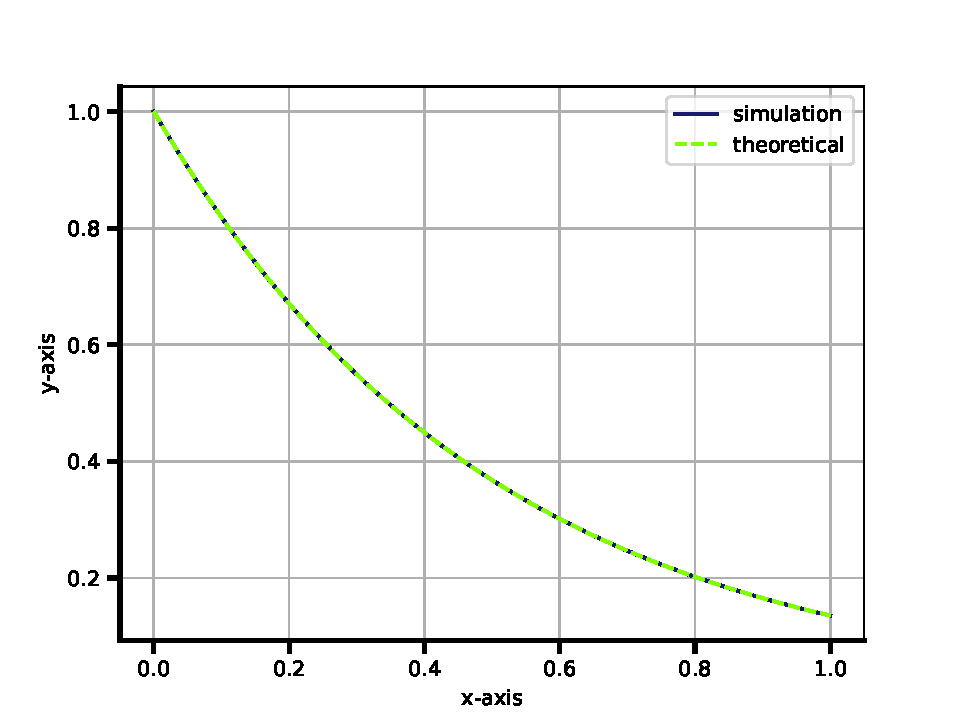
\includegraphics[width=0.7\columnwidth]{figs/fig.pdf}
\end{figure}

\end{document}
